\chapter{Benchmark}\label{experiment}

This chapter consists of four sections. First, we try to outline what a good explanation should fulfill. Then, we tackle the current problem of high computational resource utilization of the current solution. In the third section, we construct a quantitative benchmark, choosing suitable metrics alongside brief reasoning and evidence behind our choice. In the last section, we conduct a subjective evaluation by a domain expert using a previously established approach.

We will use implementation from popular XAI-oriented machine learning libraries, \texttt{captum} (Occlusion, Composite-LRP), \texttt{torch-cam} (CAM) and \texttt{pytorch-grad-cam} (HiResCAM, GradCAM++, ScoreCAM, AblationCAM). All three libraries are publicly available on \texttt{github} and provide convenient interfaces, which we can easily unify in our pipeline.

\section{What makes a good explanation?}

\emph{Unfortunately, “explainability” is a nebulous and elusive concept that is hard to target.} \cite{explainability-hard}
\newline
\noindent

Contemporary research does not provide a unified approach to define the "goodness" of an explanation. There are attempts to propose a set of properties a good explainability method should fulfill, but they are not aligned \cite{xai-functionality-grounded, explainability-hard, xai-meta-survey, xai-zhou-survey}. Moreover, some studies present contradictory results, rendering objective conclusions even more challenging \cite{xai-zhou-survey}. According to Doshi-Velez in \cite{xai-doshi}, "the field is crowded with evaluation methods, and there is no consensus on which are the “right” ones. Much less, there is not even agreement on which criteria should be evaluated.". The challenge lies in the absence of ground truth for an explanation, and therefore, we have no objective measure of grading the explanations \cite{xai-zhou-survey}. However, by carefully choosing metrics, we can avoid so-called "anecdotal evidence" and argue that certain explainability methods are sufficient given the audience and use case \cite{xai-anecdotal-evidence}. We believe that for an explanation to be applicable to our use-case of generating slide-level explanations, it needs to be:

\begin{enumerate}
    \item Performant: This is the main bottleneck of the current solution. We do not care how good a method is without reasonable performance since it cannot be utilized for practical purposes.
    \item Faithful: Ideally, we want to ensure that the explainability method only highlights the relevant parts of the input tile.
    \item Useful: We need the explanations to be presented to domain experts so that it is understandable for them. If they do not understand the explanation, it is of little value. 
\end{enumerate}

\section{Computational performance}

For the method to actively assist pathologists, the explanations must be computed fast enough not to disrupt his workflow.
The main problem of the existing approach using Occlusion-based saliency is to generate explanations for an entire slide in a reasonable time.
The current solution employs \texttt{python} implementation from the \texttt{captum} package.
The problem with Occlusion is two-fold; either we perform one forward pass with the occluded tile at a time, needing XXX synchronous forward passes, or we batch several occluded tiles together, drastically raising GPU memory costs for a single forward pass.
To tackle this problem from both perspectives --- we first measure the time required to produce a single explanation and then observe how much GPU memory it needs.

\subsection*{Time efficiency}

 We let each method fully explain the averagely-sized WSI of 1499 tiles from the test set.
 Although we aim to achieve good slide-level performance, we measure the time required for individual tile-level explanations instead.
 During the generation of slide-level explanations, there are a lot of auxiliary operations to stitch tile-level saliency maps together.
 The method and its implementation are not responsible for these operations.
 We include this overhead if we measure the time required to generate slide-level saliency maps.
 Since modern machine-learning frameworks typically employ parallel processing using multiple CPU cores, this can lead to resource locks, negatively affecting a method's performance if we were looking at the required slide-level time.
 Another reason to measure the required time for tile-level explanations is resource saving.
 We want to take multiple unit measurements and see their mean and variance since momentary factors of the machine environment can influence a single data point. 
 By taking multiple data points, we are hedging ourselves against these factors.
 If we were measuring the slide-level performance, it would be notably more time-and-resource intensive, blocking resources from other students and colleagues from the RationAI group.

 We performed each run on a machine with $8$ cores, $16$GB of RAM, and a single NVIDIA A40 GPU card with $48$GB of memory.
 For Occlusion, we used a batch size of $200$ perturbed tiles, the same settings used in the production deployment.
 Other methods do not offer such an option. We repeatedly fed each method a single tile and measured the time difference between the start and end of the computation.
 After the method call, we inserted a \texttt{torch.cuda.synchronize} call to ensure all computation on GPU is finished before taking the end-of-computation timestamp.
 We present the results in \myref{Table}{tab:comp-time}.

\begin{table}
\centering
\ra{1.2}
\begin{tabular}{@{} l c c c @{}}\toprule
Method & Avg. time per tile (s) & Time for slide (s) & Expected largest slide time (m) \\ 
\midrule
CAM           & $0.04 \pm 0.04$ & $59.45$    & $2.73$ \\
GradCAM++     & $0.08 \pm 0.00$ & $131.88$   & $6.05$ \\
HiResCAM      & $0.08 \pm 0.00$ & $131.95$   & $6.06$ \\
Composite-LRP & $0.11 \pm 0.00$ & $178.829$  & $8.21$ \\
\textbf{Occlusion}     & $1.06 \pm 0.00$ & $1612.70$  & $74.07$ \\
AblationCAM   & $9.72 \pm 0.00$ & $14583.50$ & $669.82$ \\
ScoreCAM      & $9.76 \pm 0.00$ & $14629.98$ & $671.96$ \\
\bottomrule
\end{tabular}
\caption{
Time efficiency of overviewed XAI methods.
Methods are ordered from the fastest to the slowest.
Entry for Occlusion is in bold to visually delimit the methods into faster and slower than the current solution.
Unsurprisingly, methods that require a single pass to compute activation maps' importance were the fastest, while the methods perturbing either input or model internals scored slower since they require multiple forward passes to estimate the importance.
This could be solved, as in the case of Occlusion, by batching multiple perturbed inputs together, but the libraries do not offer such an option.
Even then, we would arrive at a different problem; such batching requires tremendous GPU capacity.
The third column represents the estimated time to explain the largest slide from the test split to give a current worst-case scenario of $4131$ tiles-per-slide outlook.
}
\label{tab:comp-time}
\end{table}

\myref{Table}{tab:comp-time} shows the superiority of CAM methods, which require a single forward pass to compute the saliency maps.
Unsurprisingly, ScoreCAM scored the worst.
This stems from the fact that for each of the $512$ activation maps of the last layer of our model, ScoreCAM runs a separate forward pass with a perturbed input tile.
The problem of multiple forward passes is tamed by batching in the case of Occlusion, where most of the overhead comes from the creation of perturbed tiles.
What surprised us was the time AblationCAM needed to compute a single explanation.
\myref{Equation}{eq:ablation-cam-importance-weight} shows that the importance weights in the case of AblationCAM are computed by perturbing models internals --- systematically zeroing out activations across layer units.
In the case of our model, computing importance weight for unit $k$ means setting the pooled activation $a^k$ to zero --- output $y^c_k$ is simply a linear combination of pooled activations, omitting the $a^k$, which we would expect to be computed reasonably fast.

Since both AblationCAM and ScoreCAM scored notably worse than Occlusion and did not bring us closer to finding a performant XAI method, we decided not to include them in further benchmarks.

\subsection*{GPU utilization}

Modern GPUs offer the possibility of simultaneous execution of multiple processes on the same card instance.
The demand a method places on GPU resources is crucial for production deployment.
High GPU utilization by one method can limit the number of processes that can run in parallel, which, in turn, may increase deployment costs due to the need for additional GPU cards.
Since neural networks are generally expensive in terms of computational power, their usage inevitably leads to increased carbon emissions.
Sustainability, nowadays a crucial concern in technology development and deployment, should be thoughtfully weighed when considering the future use and advancement of deep learning models.
We are not aware of any previous work trying to focus on GPU utilization of explainability methods, but given EU regulations on AI from \myref{Section}{sec:need-for-xai}, we believe that it should be evaluated accordingly.
Not considering those requirements could negatively affect deployed models since being unable to facilitate given restrictions may require them to be brought down.

Like the Time Efficiency metric, we let each method explain a single WSI of $1499$ tiles.
We monitor the GPU usage by running the \texttt{nvidia-smi} executable in a separate process, forwarding its output every $500$ milliseconds to a CSV file.
\myref{Table}{tab:gpu-util} presents the average utilization of a single A40 GPU card, while computing the explanations.
Note that we cannot exactly distinguish which portion of the GPU memory the XAI method uses since we also store the model on GPU.
For this reason, we conducted one run without computing any explanations to serve as a baseline.
We did all of the runs using a batch size of one in an attempt not to discriminate any method.
We expect all methods to score better than Occlusion since none relies on internal batching.

The results in \myref{Table}{tab:gpu-util} confirm our expectations that none of the methods except Occlusion noticeably exhaust the GPU.
Therefore, we can run multiple processes simultaneously on a single card instance.
Moreover, all methods but Occlusion can be sufficiently run on the smallest GPU the RationAI group has at hand, having a capacity of $10$GB.
\begin{table}
\centering
\ra{1.2}
\begin{tabular}{@{} l c c @{}}\toprule
Method & Absolute GPU utilization (MB) & Relative Overhead (MB) \\ 
\midrule
-             & $910$        & -       \\
CAM           & $1084$       & $174$   \\
GradCAM++     & $1578$       & $668$   \\
HiResCAM      & $1578$       & $668$   \\
Composite-LRP & $2476$       & $1566$  \\
\textbf{Occlusion} & $36308$ & $35398$ \\
\bottomrule
\end{tabular}
\caption{
GPU utilization of overviewed XAI methods. We use mode instead of mean, as we observed that after two GPU memory utilization snapshots, the number stays the same up until the end of the benchmark. Column Absolute GPU utilization captures the raw output of \texttt{nvidia-smi} command, while column Relative Overhead corresponds to the additional consumed memory on top of the normal model's requirements. All values are reported in megabytes. All methods scored notably better than Occlusion, which we attribute mainly to not running batched forward passes. CAM achieved the lowest utilization since it only multiplies activation maps with FC layer weights. GradCAM++ and HiResCAM need to compute and retain certain gradients, which require more memory than vanilla pass. Composite-LRP runs one full backward pass equivalent and needs to retain forward pass activations to compute neuron relevance.
}
\label{tab:gpu-util}
\end{table}


\section{Quantitative evaluation}

This section covers several entrenched metrics that capture our desired traits of explainability methods.
We build on the work of \cite{gallo} by incorporating state-of-the-art metrics that address the limitations of previous approaches.
Refining previously used metrics aims to provide a more robust and reliable benchmark for evaluating our methods, aligning the quantitative assessment more closely with domain-specific boundaries and expectations.

\subsection*{Faithfulness}

An established approach to assess whether the explainability method points to the relevant part of the input is to perturb the image, such that we remove features perceived as important by the model and back-fill removed areas with certain fixed value --- similar to how occlusion estimates feature importance --- and observe how model's confidence changes.
However, the literature suggests that this perturbation approach, which involves filling the removed areas with zeros or the mean pixel value, could be flawed.
The perturbed input might include artifacts that induce a shift in the data distribution, compromising the reliability of such metrics since we cannot tell to what extent the change in the model's confidence stems from introduced artifacts compared to the initial relevance of removed features \cite{roar}.

Experiments in \cite{gallo} utilize methods prone to introducing such unintentional artifacts.
Notably, Occlusion and Deep-Taylor Decomposition \cite{xai-dtd} received the highest scores.
This is aligned with the observation by Hsieh et al. in \cite{xai-hsieh-occ-dtd} --- that such metrics may favor methods that rely on the same mechanism when estimating the importance of input features.
Since Occlusion estimates feature importance by a drop in the model's confidence by perturbing the input image with a patch --- when we later remove the region corresponding to a high attribution, the model's score will inevitably drop.
Employed metrics (Causal Deletion \cite{xai-causal-deletion} and Area Over Perturbation Curve \cite{xai-aopc}) also did not produce aligned results, confirming findings in \cite{roar}.

Hooker et al. \cite{roar} introduced an alternative metric known as Remove and Retrain (ROAR), which involves removing (zeroing out) the identified important features and then retraining the model with the modified dataset --- removing the distribution shift.
Although ROAR has gained in popularity, it has the significant downside of being computationally intensive, rendering it unacceptable for our use case.
\todo{maybe say it is shit cause we do not know to what extent the performance deterioration is thanks to bad training and removed data}
As further shown by Rong et al. in \cite{road}, ROAR does not solve the problem of the so-called \emph{class information leakage} --- phenomenon when the uniformly-valued removed region reveals relevant class info through its shape.
Rong et al. propose a method built on the foundations of ROAR, called Remove and Debias (ROAD).
Instead of retraining the model, areas after removed features are specifically imputed to reduce the risk of class information leakage \cite{road}. Refer to the original paper for mathematical intrications of information theory behind the imputation.

To evaluate the performance of our methods, ROAD iteratively removes features from the most relevant to the least (MoRF order).
After each removal, missing features are imputed using a noisy-linear imputer to reduce class information leakage \cite{road}.
For a single tile, $x$, saliency map $S$ and percentage $p$, the result of this method is a number $d$ corresponding to the drop in confidence of a model computing function $f$ when fed the imputed tile
\begin{equation}
    d = f(x) - f\bigl(\operatorname{perturb}_p(x, S)\bigr).
\end{equation}
The function $\operatorname{perturb}_p$ takes the input image $x$, saliency map $S$, and linearly imputes the areas corresponding to the top $p$ percent of most salient pixels of explanation $S$ \cite{road}.

As in one of the experiments in the original paper, we evaluate the methods at $10, 20, 30, 40$, and $50$ percent of the most salient pixels perturbed.
While other experiments in \cite{road} feature imputation up to $85$ percent, it is computationally not feasible in our setting.
Since our methods tend to cover larger areas of input tiles, imputing $85$ of the most salient pixels takes around \todo{add the final time}.
Moreover, in the production setting, the Occlusion saliency maps are thresholded to display anywhere from $55$ to $75$ of the most salient pixels.
As this thesis aims to compare the given methods against the baseline generated by Occlusion, with all these factors in mind, we decided not to extend the perturbation beyond the $50$ percent of the most salient pixels.

It is desired that the model's score should drop significantly as we start removing the features, and the rate slows down as we approach the higher percentages, signaling that the important parts were indeed removed in the beginning.
We evaluated our model using the \texttt{pytorch-grad-cam} package that provides the \texttt{NoisyLinearImputer} class.
This class is designed to handle the imputation of missing values in the same manner as the original implementation from the ROAD paper.
We did not use the original implementation from \cite{road}, as the interface did not fit into our data-processing pipeline.
\myref{Figure}{fig:road-impute} shows how the \texttt{NoisyLinearImputer} imputes removed areas.
Since this method relies on sensitivity, we will only use positive tiles from the test split of the dataset from \myref{Section}{sec:dataset}.
To see the curve of the drop in the model's confidence, refer to \myref{Figure}{fig:road-curve}.
A boxplot portraying the distribution of our results is presented in \myref{Figure}{fig:road-boxplot}.

Our findings are consistent with the study conducted by Gallo et al. \cite{gallo} --- the faithfulness metric we utilized tends to prefer techniques that identify broader, continuous regions within the input tile.
As shown in \myref{Figure}{fig:road-impute}, the tile imputed based on the explanation generated by Occlusion looks visually more distressed than the tile imputed according to the more scattered Composite-LRP method.
This explains why the HiResCAM scored worst out of all CAM-based methods since it is the most conservative in terms of how much of a tile-produced saliency map covers.
According to the \myref{Figure}{fig:road-boxplot}, CAM-based methods produce more consistent results than Occlusion-based saliency.
Similar to $\varepsilon$-LRP in \cite{gallo}, Composite-LRP performs worse than Occlusion, rendering our effort to assign different relevance rules to produce more coherent saliency maps according to \cite{lrp} unsuccessful.
An interesting observation is that upon perturbation based on saliency maps produced by Occlusion and CAM, the models' confidence does not increase, which is not the case for the rest of the methods.
We also posit that despite the authors of GradCAM++ and HiResCAM \cite{grad-cam, hires-cam} advertising their methods as more faithful than CAM/GradCAM, our results suggest otherwise.

\begin{figure}
    \begin{center}
    \begin{minipage}{1\textwidth}
      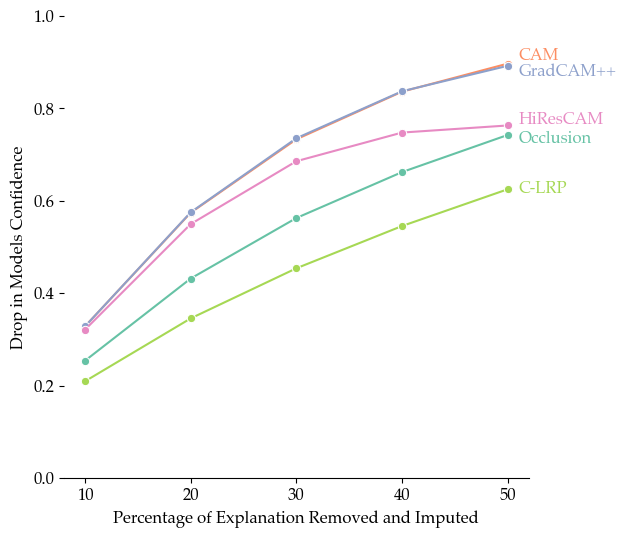
\includegraphics[width=\textwidth]{img/road-curve.png}
    \end{minipage}
    \caption{Curve visualizing mean drop in confidence of individual methods per imputed percentages of most salient pixels. Notice that looking only at the mean renders CAM and GradCAM++ as methods achieving similar performance.}
    \label{fig:road-curve}
    \end{center}
\end{figure}

\begin{figure}
    \begin{center}
    \begin{minipage}{1\textwidth}
      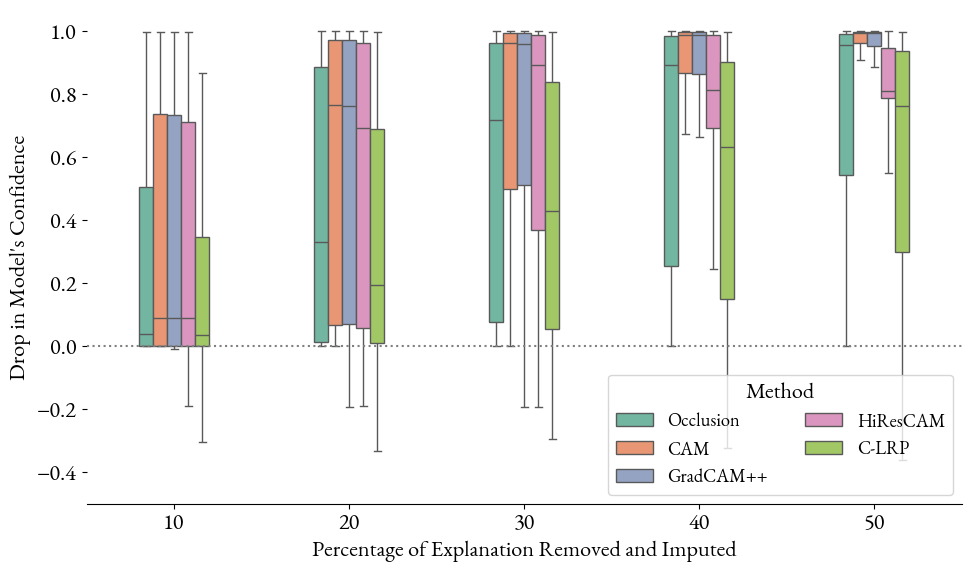
\includegraphics[width=\textwidth]{img/road-boxplot.png}
    \end{minipage}
    \caption{Boxplot of results for different percentages of ROAD method. We used the percentages from \cite{road}. ROAD ranks CAM methods over Occlusion and Composite-LRP. We can see that perturbation by CAM-based method explanations also decreases the model's confidence faster than the Occlusion method --- advocating for the CAM explanations to be more faithful. Scores for CAM methods also have less variance when significant parts of salient areas are removed. Notice the minimum values and that only CAM and Occlusion do not increase models' confidence upon evaluation of perturbed tile, while gradient-based CAMs and Composite-LRP do.}
    \label{fig:road-boxplot}
    \end{center}
\end{figure}

\begin{figure}
    \begin{center}
    \begin{minipage}{0.8\textwidth}
      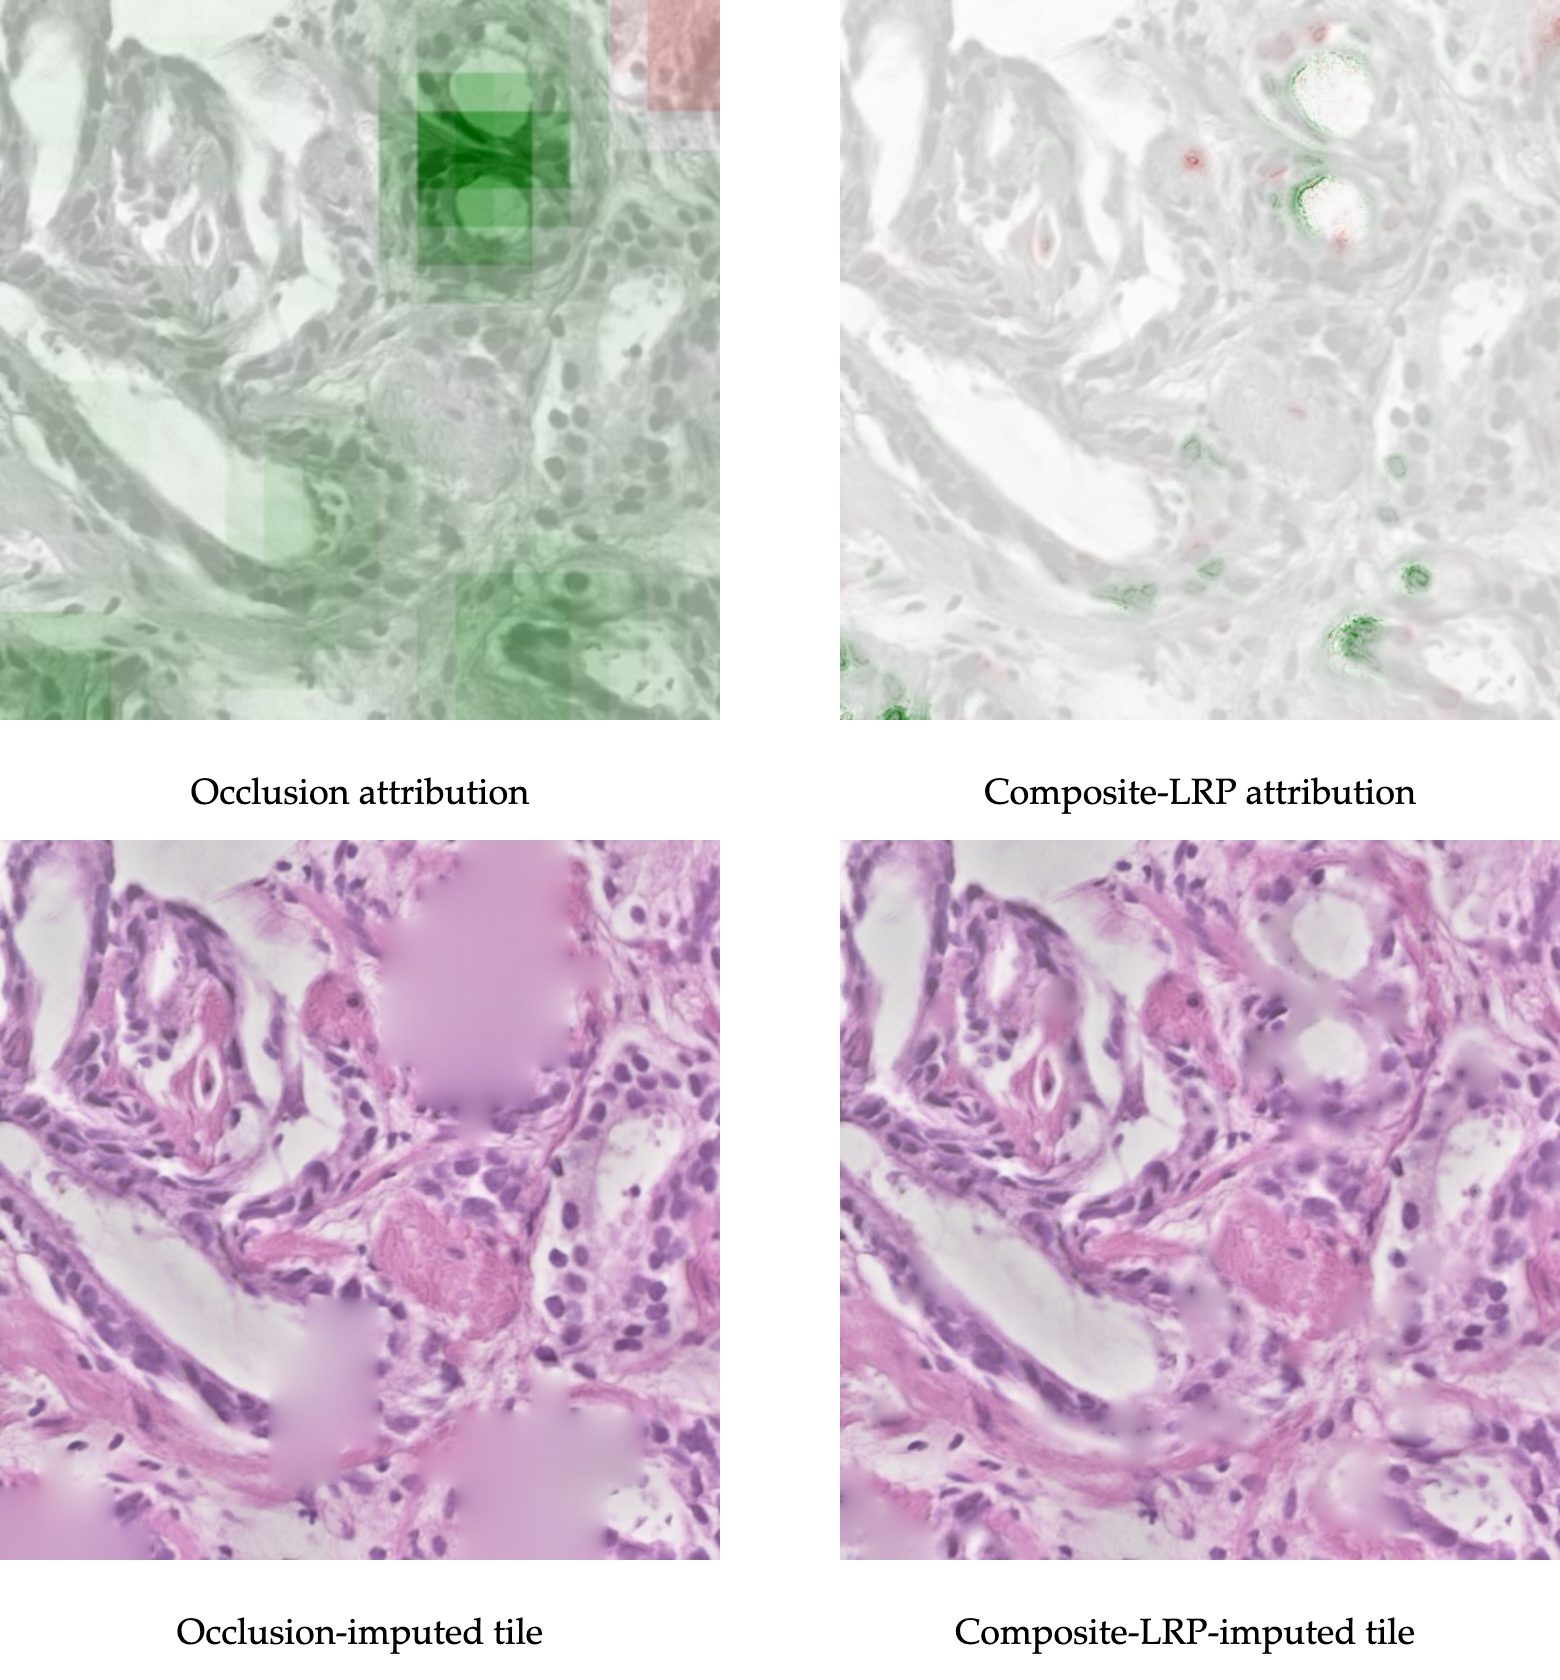
\includegraphics[width=\textwidth]{img/road-impute.png}
    \end{minipage}
    \caption{Upper row depicts attributions for Occlusion and Composite-LRP for the same tile. The bottom row shows a visualization of the tile imputed based on the $20$ percent of the most salient attribution pixels. While \texttt{NoisyLinearImputer} removes continuous regions based on the Occlusion attribution, the scattered Composite-LRP attribution and following imputation lead to a tile visually very similar to the original one. As a result, methods producing less-scattered explanations received higher scores, in agreement with results from \cite{gallo}. Images featuring attributions are presented in black and white to increase the visual contrast between the tile and the explanation.}
    \label{fig:road-impute}
    \end{center}
\end{figure}

\subsection*{Localization}

The faithfulness metric tells us how well the explainability method attributes important locations.
In addition, we want to ensure that these locations resemble what pathologists would classify as adenocarcinoma.
To measure how well the output of a given method matches the pathologists' annotation, Gallo et al. \cite{gallo} utilized the Effective Heat Ratio (EHR) \cite{ehr} metric.
EHR relies on ground truth bounding boxes, which encapsulate objects of interest.
Because of our specific use case, we argue that EHR is not the most suitable method.
Given a bounding box, by design, EHR favors methods that cover larger annotation areas with strong saliency.
This is not necessarily desired, as the bounding box only marks the rough location of cancerous tissue -- precise pixel-level borders are difficult to follow \cite{gallo, annotation-agreement} and such annotation would likely vary from pathologist to pathologist \cite{annotation-agreement}.
Therefore, EHR discriminates metrics that could potentially point to cancerous markers but do not attribute healthy surrounding tissue included in the annotation.

We will use what we consider a simpler technique called Weighting Game instead \cite{weighting-game}.
It builds upon the established Pointing Game metric \cite{pointing-game}, which looks at whether the most salient pixel falls into the bounding box.
Unlike the Pointing Game, which gives us just binary information about the accuracy of a given method, the Weighting Game calculates the ratio of the mass of the saliency map $S$ within the bounding box to the total mass of the $S$.
Compared to EHR, this does not disqualify methods that highlight smaller parts of the annotated area, and we believe it gives us a fair measure of how the explanation holds compared to the pathologist's annotation.
\myref{Figure}{fig:weighting-game-boxplot} depicts \todo{finish yapping}

\begin{figure}
    \begin{center}
    \begin{minipage}{1\textwidth}
      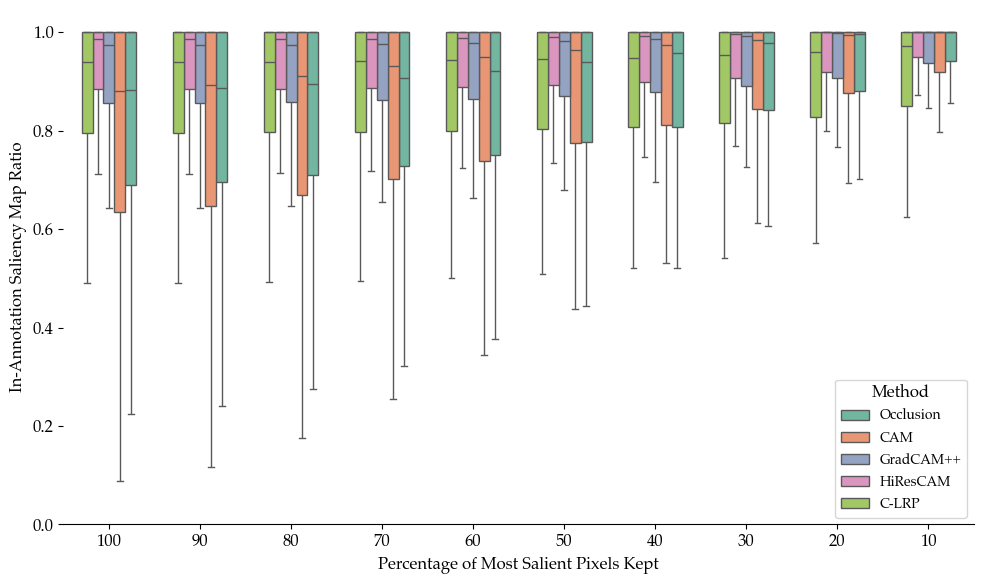
\includegraphics[width=\textwidth]{img/weighting-game-boxplot.png}
    \end{minipage}
    \caption{}
    \label{fig:weighting-game-boxplot}
    \end{center}
\end{figure}

\subsection*{Usefulness}

The usefulness of an explanation in the context of machine learning and deep learning models is inherently subjective, as it can vary significantly depending on the individual's perspective and context --- the audience's background, expertise, and purpose of use all play critical roles in determining the perceived utility of an explanation \cite{xai-doshi} --- something hard to capture by a quantitative metric.

Luckily, we know that a solution based on Occlusion produces semantically correct explanations aligned with features recognized by pathologists \cite{gallo}.
Therefore, we will reuse the metric from Subsection LOCALIZATION and take $55$\% most salient occlusion explanation as our bounding box.
Since such "annotations" do not represent ground truth, we do not perceive this metric as adding to the truthfulness.
Instead, its purpose is twofold.
First, it guides our selection of which explainability methods to present to a pathologist, allowing us to prioritize explanations that align most closely with the established Occlusion baseline.
Second, it enables us to evaluate how the pathologist subjectively perceives candidate explainability techniques relative to the established understanding and acceptance of Occlusion-based saliency maps.
\myref{Figure}{fig:occ-weighting-game-boxplot} depicts \todo{finish yapping}

\begin{figure}
    \begin{center}
    \begin{minipage}{1\textwidth}
      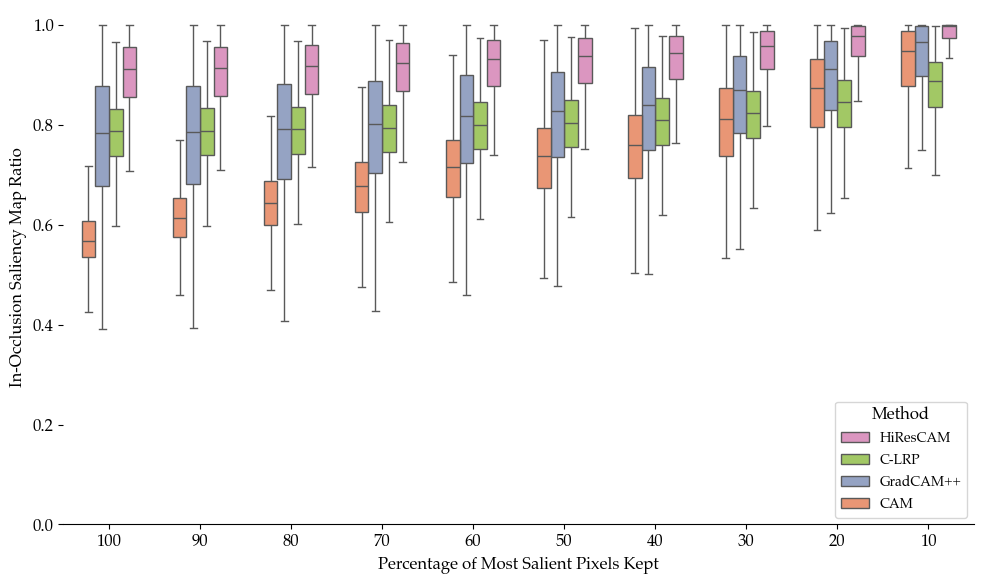
\includegraphics[width=\textwidth]{img/occlusion-weighting-game-boxplot.png}
    \end{minipage}
    \caption{}
    \label{fig:occ-weighting-game-boxplot}
    \end{center}
\end{figure}

\section{Domain expert assessment}

This section presents qualitative evaluation of produced explanations by domain expert. We replicate experiment from []. What follows is assessment from Dr. Nenutil on how are explanations perceived from POV of a clinician.
